% Options for packages loaded elsewhere
\PassOptionsToPackage{unicode}{hyperref}
\PassOptionsToPackage{hyphens}{url}
\PassOptionsToPackage{dvipsnames,svgnames,x11names}{xcolor}
%
\documentclass[
  letterpaper,
  DIV=11,
  numbers=noendperiod]{scrartcl}

\usepackage{amsmath,amssymb}
\usepackage{iftex}
\ifPDFTeX
  \usepackage[T1]{fontenc}
  \usepackage[utf8]{inputenc}
  \usepackage{textcomp} % provide euro and other symbols
\else % if luatex or xetex
  \usepackage{unicode-math}
  \defaultfontfeatures{Scale=MatchLowercase}
  \defaultfontfeatures[\rmfamily]{Ligatures=TeX,Scale=1}
\fi
\usepackage{lmodern}
\ifPDFTeX\else  
    % xetex/luatex font selection
\fi
% Use upquote if available, for straight quotes in verbatim environments
\IfFileExists{upquote.sty}{\usepackage{upquote}}{}
\IfFileExists{microtype.sty}{% use microtype if available
  \usepackage[]{microtype}
  \UseMicrotypeSet[protrusion]{basicmath} % disable protrusion for tt fonts
}{}
\makeatletter
\@ifundefined{KOMAClassName}{% if non-KOMA class
  \IfFileExists{parskip.sty}{%
    \usepackage{parskip}
  }{% else
    \setlength{\parindent}{0pt}
    \setlength{\parskip}{6pt plus 2pt minus 1pt}}
}{% if KOMA class
  \KOMAoptions{parskip=half}}
\makeatother
\usepackage{xcolor}
\setlength{\emergencystretch}{3em} % prevent overfull lines
\setcounter{secnumdepth}{-\maxdimen} % remove section numbering
% Make \paragraph and \subparagraph free-standing
\makeatletter
\ifx\paragraph\undefined\else
  \let\oldparagraph\paragraph
  \renewcommand{\paragraph}{
    \@ifstar
      \xxxParagraphStar
      \xxxParagraphNoStar
  }
  \newcommand{\xxxParagraphStar}[1]{\oldparagraph*{#1}\mbox{}}
  \newcommand{\xxxParagraphNoStar}[1]{\oldparagraph{#1}\mbox{}}
\fi
\ifx\subparagraph\undefined\else
  \let\oldsubparagraph\subparagraph
  \renewcommand{\subparagraph}{
    \@ifstar
      \xxxSubParagraphStar
      \xxxSubParagraphNoStar
  }
  \newcommand{\xxxSubParagraphStar}[1]{\oldsubparagraph*{#1}\mbox{}}
  \newcommand{\xxxSubParagraphNoStar}[1]{\oldsubparagraph{#1}\mbox{}}
\fi
\makeatother


\providecommand{\tightlist}{%
  \setlength{\itemsep}{0pt}\setlength{\parskip}{0pt}}\usepackage{longtable,booktabs,array}
\usepackage{calc} % for calculating minipage widths
% Correct order of tables after \paragraph or \subparagraph
\usepackage{etoolbox}
\makeatletter
\patchcmd\longtable{\par}{\if@noskipsec\mbox{}\fi\par}{}{}
\makeatother
% Allow footnotes in longtable head/foot
\IfFileExists{footnotehyper.sty}{\usepackage{footnotehyper}}{\usepackage{footnote}}
\makesavenoteenv{longtable}
\usepackage{graphicx}
\makeatletter
\newsavebox\pandoc@box
\newcommand*\pandocbounded[1]{% scales image to fit in text height/width
  \sbox\pandoc@box{#1}%
  \Gscale@div\@tempa{\textheight}{\dimexpr\ht\pandoc@box+\dp\pandoc@box\relax}%
  \Gscale@div\@tempb{\linewidth}{\wd\pandoc@box}%
  \ifdim\@tempb\p@<\@tempa\p@\let\@tempa\@tempb\fi% select the smaller of both
  \ifdim\@tempa\p@<\p@\scalebox{\@tempa}{\usebox\pandoc@box}%
  \else\usebox{\pandoc@box}%
  \fi%
}
% Set default figure placement to htbp
\def\fps@figure{htbp}
\makeatother

\KOMAoption{captions}{tableheading}
\makeatletter
\@ifpackageloaded{tcolorbox}{}{\usepackage[skins,breakable]{tcolorbox}}
\@ifpackageloaded{fontawesome5}{}{\usepackage{fontawesome5}}
\definecolor{quarto-callout-color}{HTML}{909090}
\definecolor{quarto-callout-note-color}{HTML}{0758E5}
\definecolor{quarto-callout-important-color}{HTML}{CC1914}
\definecolor{quarto-callout-warning-color}{HTML}{EB9113}
\definecolor{quarto-callout-tip-color}{HTML}{00A047}
\definecolor{quarto-callout-caution-color}{HTML}{FC5300}
\definecolor{quarto-callout-color-frame}{HTML}{acacac}
\definecolor{quarto-callout-note-color-frame}{HTML}{4582ec}
\definecolor{quarto-callout-important-color-frame}{HTML}{d9534f}
\definecolor{quarto-callout-warning-color-frame}{HTML}{f0ad4e}
\definecolor{quarto-callout-tip-color-frame}{HTML}{02b875}
\definecolor{quarto-callout-caution-color-frame}{HTML}{fd7e14}
\makeatother
\makeatletter
\@ifpackageloaded{caption}{}{\usepackage{caption}}
\AtBeginDocument{%
\ifdefined\contentsname
  \renewcommand*\contentsname{Table of contents}
\else
  \newcommand\contentsname{Table of contents}
\fi
\ifdefined\listfigurename
  \renewcommand*\listfigurename{List of Figures}
\else
  \newcommand\listfigurename{List of Figures}
\fi
\ifdefined\listtablename
  \renewcommand*\listtablename{List of Tables}
\else
  \newcommand\listtablename{List of Tables}
\fi
\ifdefined\figurename
  \renewcommand*\figurename{Figure}
\else
  \newcommand\figurename{Figure}
\fi
\ifdefined\tablename
  \renewcommand*\tablename{Table}
\else
  \newcommand\tablename{Table}
\fi
}
\@ifpackageloaded{float}{}{\usepackage{float}}
\floatstyle{ruled}
\@ifundefined{c@chapter}{\newfloat{codelisting}{h}{lop}}{\newfloat{codelisting}{h}{lop}[chapter]}
\floatname{codelisting}{Listing}
\newcommand*\listoflistings{\listof{codelisting}{List of Listings}}
\makeatother
\makeatletter
\makeatother
\makeatletter
\@ifpackageloaded{caption}{}{\usepackage{caption}}
\@ifpackageloaded{subcaption}{}{\usepackage{subcaption}}
\makeatother

\usepackage{bookmark}

\IfFileExists{xurl.sty}{\usepackage{xurl}}{} % add URL line breaks if available
\urlstyle{same} % disable monospaced font for URLs
\hypersetup{
  pdftitle={Lab 6: Inference for Two Independent Means: Independent Samples t-test},
  colorlinks=true,
  linkcolor={blue},
  filecolor={Maroon},
  citecolor={Blue},
  urlcolor={Blue},
  pdfcreator={LaTeX via pandoc}}


\title{Lab 6: Inference for Two Independent Means: Independent Samples
t-test}
\author{}
\date{}

\begin{document}
\maketitle


\begin{center}\rule{0.5\linewidth}{0.5pt}\end{center}

\subsection{Part 1: Scenario \&
Overview}\label{part-1-scenario-overview}

In the previous lab, we performed a \textbf{\emph{one-sample t-test}} to
determine if the average weight loss for individuals in the incentive
group was significantly different from the known population mean of 10
pounds. In this lab, we will perform a \textbf{\emph{two-sample t-test}}
to determine if there is a significant difference in average weight loss
between the incentive group and the control group.

Here is the research question we will be investigating:

\begin{tcolorbox}[enhanced jigsaw, opacityback=0, colbacktitle=quarto-callout-tip-color!10!white, colframe=quarto-callout-tip-color-frame, leftrule=.75mm, bottomtitle=1mm, titlerule=0mm, title=\textcolor{quarto-callout-tip-color}{\faLightbulb}\hspace{0.5em}{Research Question}, opacitybacktitle=0.6, toptitle=1mm, colback=white, bottomrule=.15mm, rightrule=.15mm, breakable, arc=.35mm, toprule=.15mm, left=2mm, coltitle=black]

Does the new weight loss program with financial incentives result in a
significantly higher average weight loss than the traditional weight
loss program without financial incentives?

\end{tcolorbox}

Here is the scenario to that we will be working with:

A fitness center wants to determine if using financial incentives is
associated with greater weight loss among participants. The fitness
center has a new weight loss program that offers financial incentives to
individuals who meet their weight loss goals. The center wants to
determine if the new program is more effective than the traditional
weight loss program that does not offer financial incentives.

\textbf{Study Design:} The researchers recruited 38 individuals who
wanted to lose weight and randomly assigned them to either an incentive
group (given financial incentives) or a control group (not given any
financial incentives). After 4 months, the researchers recorded the
amount of weight lost (before - after) by each individual. Three months
after the initial 4 months, they also recorded the weight lost by each
individual again to see if the weight loss was maintained. However,
financial incentives were only given during the first 4 months.

\begin{tcolorbox}[enhanced jigsaw, opacityback=0, colbacktitle=quarto-callout-note-color!10!white, colframe=quarto-callout-note-color-frame, leftrule=.75mm, bottomtitle=1mm, titlerule=0mm, title=\textcolor{quarto-callout-note-color}{\faInfo}\hspace{0.5em}{Learning Objectives}, opacitybacktitle=0.6, toptitle=1mm, colback=white, bottomrule=.15mm, rightrule=.15mm, breakable, arc=.35mm, toprule=.15mm, left=2mm, coltitle=black]

By the end of this lab, you should be able to:

\begin{itemize}
\tightlist
\item
  State null and alternative hypotheses for an independent samples
  t-test.
\item
  Perform an independent samples t-test in SPSS.
\item
  Interpret the results of an independent samples t-test in APA style.
\end{itemize}

\end{tcolorbox}

\subsubsection{Stating Hypotheses}\label{stating-hypotheses}

Null Hypothesis: There is no difference in average weight loss between
individuals in the incentive group and the control group.

In symbols: \(H_0: \mu_1-\mu_2 = 0\)

Alternative Hypothesis: There is a difference in average weight loss
between individuals in the incentive group and the control group.

In symbols: \(H_1: \mu_1-\mu_2 \neq 0\)

\subsubsection{Checking Assumptions}\label{checking-assumptions}

There are two main assumptions to consider before running a one-sample
t-test:

\begin{itemize}
\item
  \textbf{Independence:} The individuals in the study must be
  independent, meaning that each participant or observation belongs to
  only one group. In this study, the individuals were randomly assigned
  to either the incentive or control group, so this assumption is
  satisfied.
\item
  \textbf{Normality:} The distribution of the dependent variable (weight
  loss) should be approximately normal for each group. We will check
  this assumption using visualizations and summary statistics in the
  next section. With large samples (n \textgreater{} 30), the t-test is
  robust to violations of normality, but with smaller samples, it is
  important to check this assumption.
\item
  \textbf{No Significant Outliers:} The dependent variable should not
  have any significant outliers. We will check for outliers using box
  plots in the next section.
\item
  \textbf{Homogeneity of Variance:} The variance of the dependent
  variable (weight in this case) should be approximately equal for both
  groups.
\end{itemize}

\begin{center}\rule{0.5\linewidth}{0.5pt}\end{center}

\subsection{Part 2: The Data}\label{part-2-the-data}

\subsubsection{Importing Data into SPSS}\label{importing-data-into-spss}

The data set is available in the following link. Download the data.

\href{datasets/weightLoss.csv}{WeightLoss}.

After downloading the dataset, import it into SPSS, using the following
steps:

\textbf{File \textgreater{} Import Data \textgreater{} CSV
Data\ldots{}}, browse to the file location, and click \textbf{OK} on the
import wizard (accept the default settings).

Make sure the measurement scales are set as follows: \texttt{WeightLoss}
= Scale, \texttt{Group} = Nominal, \texttt{Month7Loss} = Scale.

See the screenshot below for reference:

\begin{center}
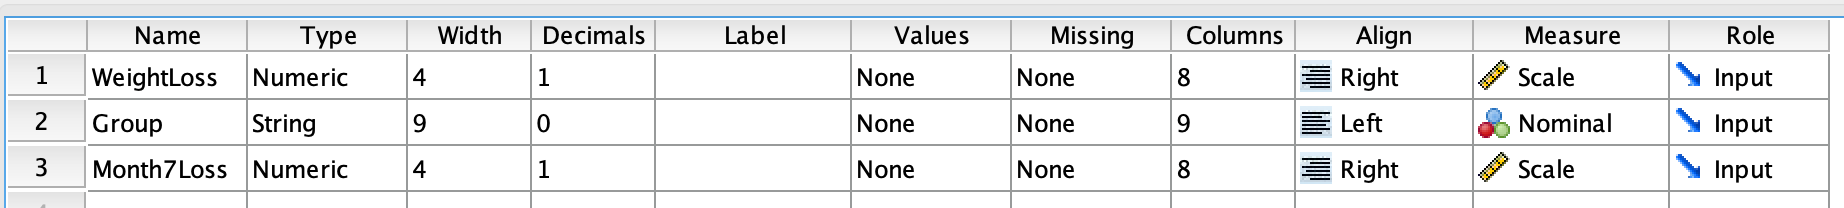
\includegraphics[width=7.69792in,height=\textheight,keepaspectratio]{images/lab5im2.png}
\end{center}

\begin{tcolorbox}[enhanced jigsaw, opacityback=0, colbacktitle=quarto-callout-tip-color!10!white, colframe=quarto-callout-tip-color-frame, leftrule=.75mm, bottomtitle=1mm, titlerule=0mm, title=\textcolor{quarto-callout-tip-color}{\faLightbulb}\hspace{0.5em}{variable Description}, opacitybacktitle=0.6, toptitle=1mm, colback=white, bottomrule=.15mm, rightrule=.15mm, breakable, arc=.35mm, toprule=.15mm, left=2mm, coltitle=black]

The variable description is as follows:

\begin{itemize}
\item
  \textbf{\emph{Group}} = Whether someone was in the Incentive or
  Control group. \textbf{0=Control group, 1=Incentive group}.
\item
  \textbf{\emph{Weightloss}} = The amount of weight lost by each
  individual at the 4-month follow-up.
\item
  \textbf{\emph{Month7Loss}} = The amount of weight lost by each
  individual at the 7-month follow-up
\end{itemize}

\end{tcolorbox}

Click on data view to confirm that you have 38 individuals in the data
set. The \texttt{WeightLoss} variable is calculated as the difference
between the weight before and after the 4-month period. Negative values
(e.g., case 14) indicate that the individual gained weight.

The goal is to determine if the average initial weight loss
(\texttt{Weightloss}) for individuals in the incentive group is
significantly different from the average weight loss for individuals in
the control group.

\begin{center}\rule{0.5\linewidth}{0.5pt}\end{center}

\subsection{Part 3: Exploratory
Analysis}\label{part-3-exploratory-analysis}

Before running the t-test, we will perform some exploratory analysis to
understand any patterns/trends in the data.

\subsubsection{Summary Statistics}\label{summary-statistics}

First, we want to generate a table of summary statistics for the
\texttt{WeightLoss} variable. Run the following steps:

Analyze \textgreater{} Compare Means and Proportions \textgreater{}
Means.

The following dialog box should appear:

\begin{center}
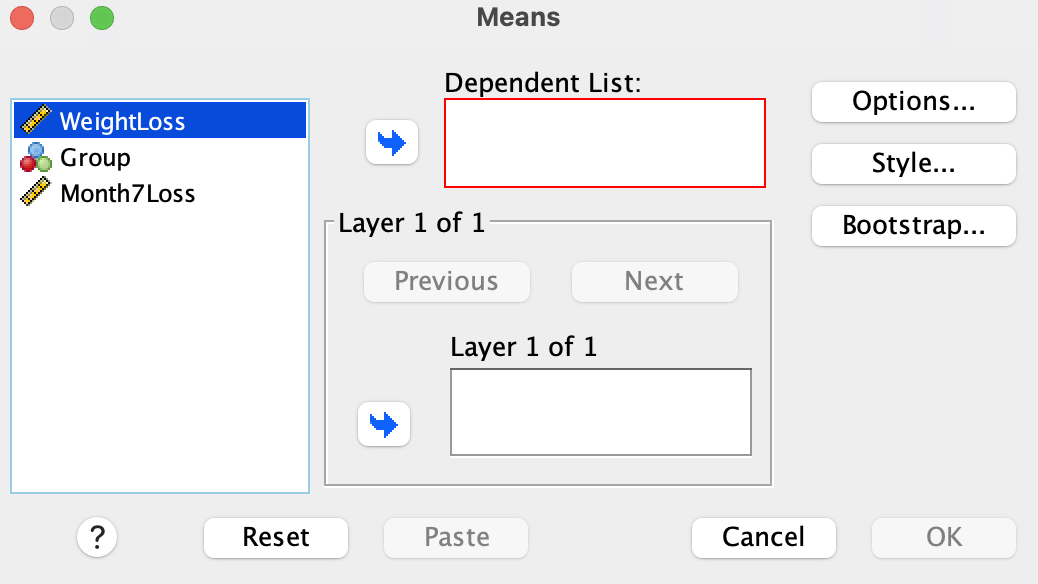
\includegraphics[width=6.25in,height=\textheight,keepaspectratio]{images/lab6im1.png}
\end{center}

Send the \texttt{WeightLoss} variable into the \textbf{Dependent List}
box and the \texttt{Group} variable into the \textbf{Independent List}
box. See below:

\begin{center}
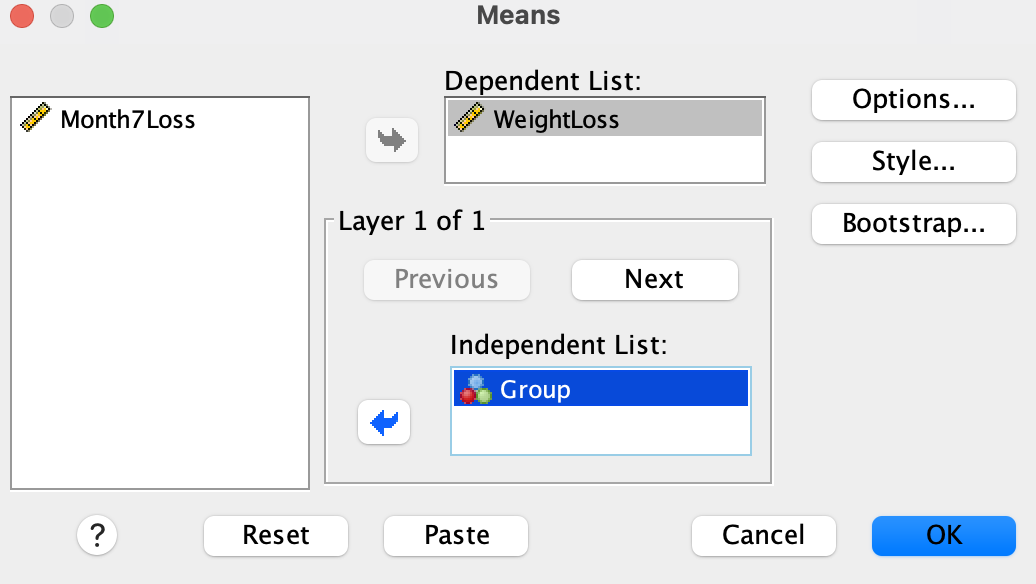
\includegraphics[width=6.25in,height=\textheight,keepaspectratio]{images/lab6im2.png}
\end{center}

Click \textbf{OK}.

Optionally, you may click on \textbf{Options} during the variable
selection to select step above for additional summary statistics (e.g.,
median, range, etc.) to include in the output.

You should see the following table in the output window:

\begin{center}
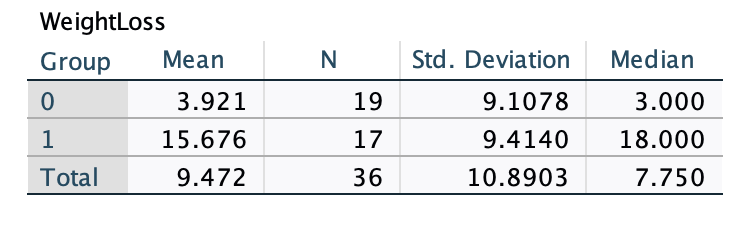
\includegraphics[width=6.25in,height=\textheight,keepaspectratio]{images/lab6im3.png}
\end{center}

\begin{tcolorbox}[enhanced jigsaw, opacityback=0, colbacktitle=quarto-callout-tip-color!10!white, colframe=quarto-callout-tip-color-frame, leftrule=.75mm, bottomtitle=1mm, titlerule=0mm, title=\textcolor{quarto-callout-tip-color}{\faLightbulb}\hspace{0.5em}{Output Interpretation}, opacitybacktitle=0.6, toptitle=1mm, colback=white, bottomrule=.15mm, rightrule=.15mm, breakable, arc=.35mm, toprule=.15mm, left=2mm, coltitle=black]

The table shows the the individuals in the control group (recorded as 0)
on average lost \(M = 3.921\) lbs with \(SD = 9.1\) lbs, while the
individuals in the incentive group (recorded as 1) on average lost
\(M = 15.68\) lbs with \(SD = 9.41\) lbs. Based on this information, we
can see that the variance in weight loss is similar between the two
groups, hence satisfying the assumption of homogeneity of variance.

\end{tcolorbox}

\subsubsection{Visualizations}\label{visualizations}

We can create a side-by-side box plot to visualize the distribution of
the \texttt{WeightLoss} variable for both groups. Run the following
steps:

\begin{itemize}
\tightlist
\item
  Graphs \textgreater{} Chart Builder \textgreater{} Boxplot.
\item
  Select the \textbf{Simple Boxplot} from the gallery and drag the plot
  into the \textbf{preview} window.
\item
  Drag the \texttt{WeightLoss} variable into the \textbf{Y-axis} box and
  the \texttt{Group} variable into the \textbf{X-axis} box.
\item
  Click \textbf{OK}.
\end{itemize}

Yous should see the following box plot in the output window:

\begin{center}
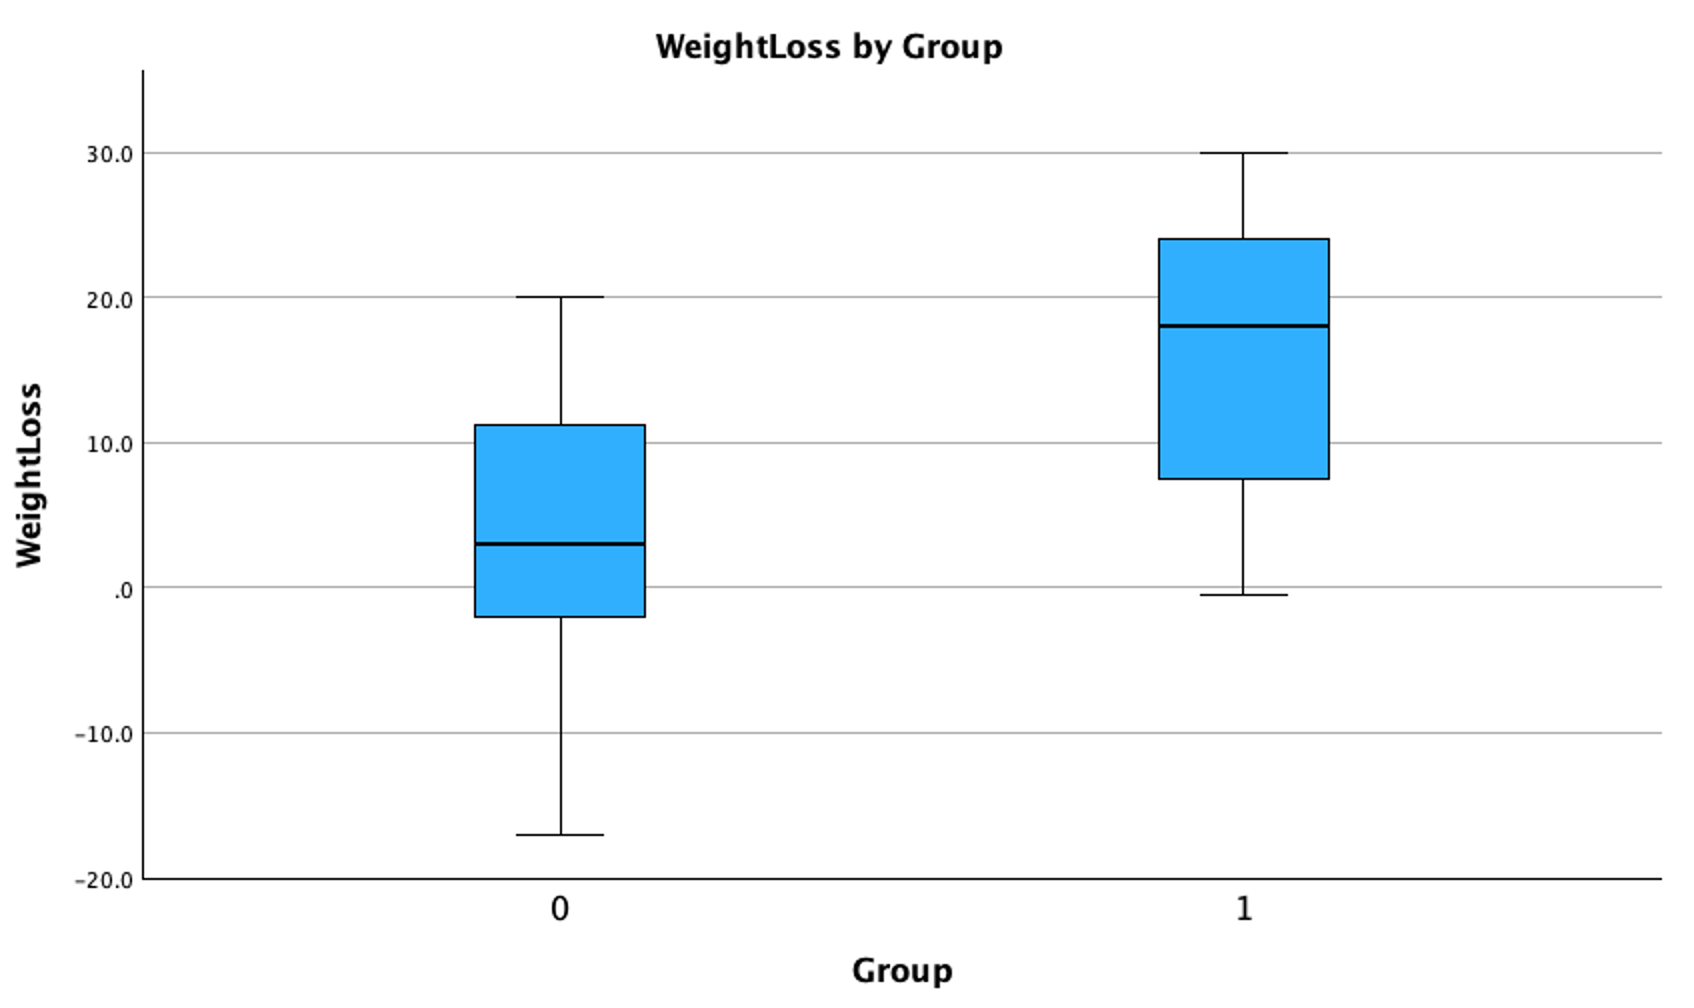
\includegraphics[width=6.25in,height=\textheight,keepaspectratio]{images/lab6im6.png}
\end{center}

\begin{tcolorbox}[enhanced jigsaw, opacityback=0, colbacktitle=quarto-callout-tip-color!10!white, colframe=quarto-callout-tip-color-frame, leftrule=.75mm, bottomtitle=1mm, titlerule=0mm, title=\textcolor{quarto-callout-tip-color}{\faLightbulb}\hspace{0.5em}{Checkpoint}, opacitybacktitle=0.6, toptitle=1mm, colback=white, bottomrule=.15mm, rightrule=.15mm, breakable, arc=.35mm, toprule=.15mm, left=2mm, coltitle=black]

How does the spread of the weight lost at the fourth month
(\texttt{WeightLoss} variable) compare between the incentive (Group 1)
and control (Group 0) groups?

\end{tcolorbox}

\begin{center}\rule{0.5\linewidth}{0.5pt}\end{center}

\subsection{Part 4: Running the t-test}\label{part-4-running-the-t-test}

To run the independent samples t-test, follow these steps:

\begin{itemize}
\tightlist
\item
  Analysis \textgreater{} Compare Means and Proportions \textgreater{}
  Independent Samples T Test.
\item
  Send the \texttt{WeightLoss} variable into the \textbf{Test
  Variable(s)} box and the \texttt{Group} variable into the
  \textbf{Grouping Variable} box. See below:
\end{itemize}

\begin{center}
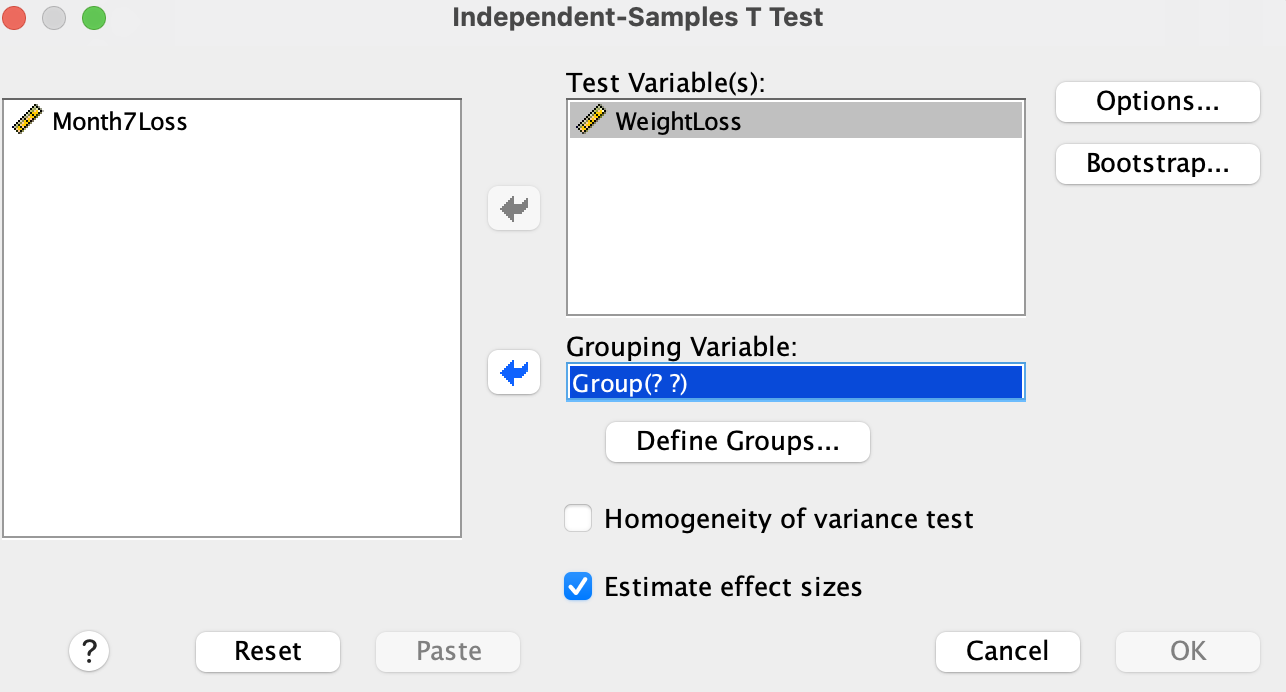
\includegraphics[width=6.25in,height=\textheight,keepaspectratio]{images/lab6im4.png}
\end{center}

\begin{itemize}
\tightlist
\item
  Next, click on \textbf{Define Groups} and enter 0 for Group 1 and 1
  for Group 2.
\item
  Click \textbf{Continue}.
\end{itemize}

The following tables should pop up in the output window:

\begin{center}
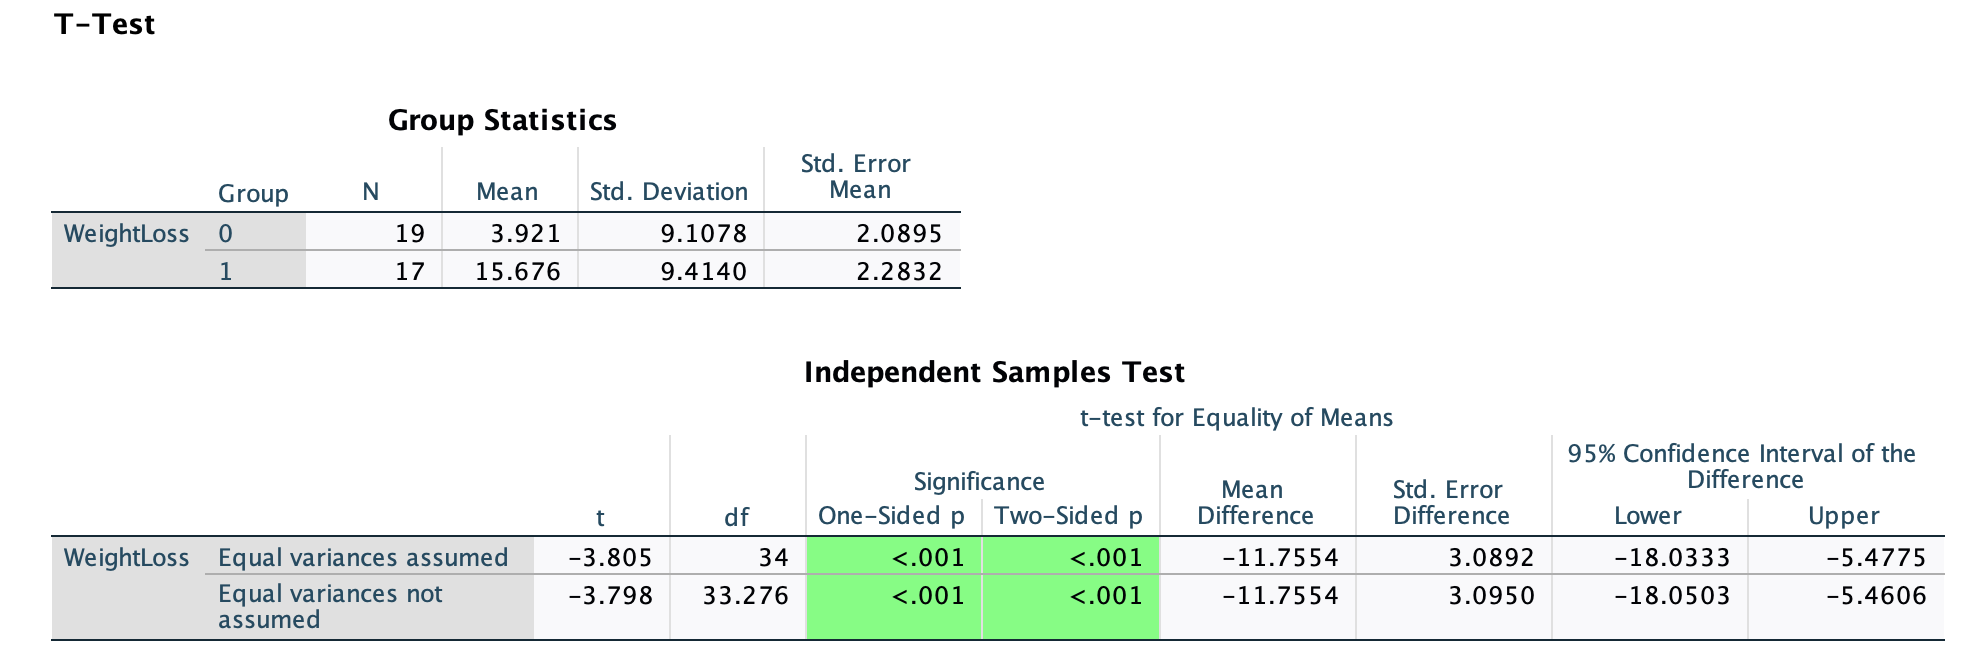
\includegraphics[width=7.8125in,height=\textheight,keepaspectratio]{images/lab6im5.png}
\end{center}

\begin{center}\rule{0.5\linewidth}{0.5pt}\end{center}

\subsection{Part 5: Output
Interpretation}\label{part-5-output-interpretation}

The output shows both summary statistics (mean, standard deviation, and
standard error) for each group and the results of the independent
samples t-test. The t-test results (second table, first row) include the
t-statistic, degrees of freedom, p-value (one-sided and two-sided), and
the confidence interval. In this case, we use the first row because it
assumes equal variances.

The P-value measures the chance (or probability) of obtaining a
difference in average weight loss of 11.75 lbs or more extreme if the
null hypothesis (average difference = 0) is true. Our obtained P-value
is extremely small (less than the significance level of 0.05), so we
reject the null hypothesis and conclude that the data provides strong
evidence to suggest that there is a difference in average weight loss
between individuals who get incentives and those who don't. In
particular, individuals who get incentives lose more weight on average
than those who do not.

The 95\% confidence interval for the difference in average weight loss
between the two groups is {[}-18.033 to -6.05{]} lbs. This means that we
are 95\% confident that the true difference in average weight loss
between the two groups is between -18.033 lbs and -6.05 lbs. Since this
confidence interval does not include 0, it provides further evidence to
reject the null hypothesis.

\begin{tcolorbox}[enhanced jigsaw, opacityback=0, colbacktitle=quarto-callout-tip-color!10!white, colframe=quarto-callout-tip-color-frame, leftrule=.75mm, bottomtitle=1mm, titlerule=0mm, title=\textcolor{quarto-callout-tip-color}{\faLightbulb}\hspace{0.5em}{APA-style Write-up}, opacitybacktitle=0.6, toptitle=1mm, colback=white, bottomrule=.15mm, rightrule=.15mm, breakable, arc=.35mm, toprule=.15mm, left=2mm, coltitle=black]

``A research report typically presents the descriptive statistics
followed by the results of the hypothesis test and the measures of
effect size (inferential statistics).'' - See p.~343 of the textbook.

Here is how to write up the results of the independent samples t-test
for our scenario above:

The participants who received financial incentives lost more weight
\((M = 15.68, SD = 9.41)\) than those who did not receive financial
incentives \((M = 3.92, SD = 9.10)\). The mean difference was
significant, \(t(36) = -3.805, p < .001, d = -1.27\).

\end{tcolorbox}

\subsection{Take-Home Lab Exercises}\label{take-home-lab-exercises}

In today's lab exercises, you will perform an \textbf{independent
samples T-test} as demonstrated in the above exploration work.

The \textbf{research question} being examined is whether in the general
population, there is a difference in average weight loss at the seventh
month (\texttt{Month7Loss}) between individuals who receive incentives
and those who don't.

\subsubsection{Question 1}\label{question-1}

What is the population of interest in the scenario? State the null and
the alternative hypotheses in words and in symbols.

\subsubsection{Question 2}\label{question-2}

Create side-by-side box plots to visualize the distribution of the
weight loss at the seventh month (\texttt{Month7Loss}) for the incentive
and the non-incentive groups. How do these distributions compare?

\subsubsection{Question 3}\label{question-3}

Run an independent samples t-test to test the whether, in the overall
population, there is a difference in average weight loss at the seventh
month between the incentive group and the non incentive group.

\begin{enumerate}
\def\labelenumi{\alph{enumi})}
\item
  What is the P-value for the two-sided test? What does this mean in the
  context of the research question?
\item
  State and interpret the 95\% confidence interval for this scenario.
\item
  What is the effect size (Cohen's d) for this test? To find this,
  please check the table near the bottom of your t-test output. How
  would you interpret this effect size in the context of the scenario at
  hand?
\end{enumerate}

\subsubsection{Question 4}\label{question-4}

Write an APA-style interpretation of the results of the independent
samples t-test performed in exercise 3 above.




\end{document}
